\chapter{Metodologia}
\label{chap:meto}
\begin{flushright}
	"Tudo o que temos de decidir é o que fazer com o tempo que nos é dado." \\
	\ \\
	(Gandalf)
\end{flushright}

De acordo com \cite{maia} metodologia é “o conjunto de métodos e técnicas aplicadas para um determinado fim. É o caminho percorrido, a maneira utilizada para atingir um objetivo”. Por certo, descreve os métodos que padronizam uma produção, visando a chegada em um resultado. Em trabalhos acadêmicos a sua importância vai além de descrever o processo de confecção do projeto mas também permite que o mesmo possa ser replicado por outros pesquisadores.

A metodologia aplicada para para o projeto toma como base o desenvolvimento de sistemas robóticos, nesse caso sendo voltada para o desenvolvimento de um sistema de movimentação robótico, presente no robô \textit{ELIR}. A divisão do projeto em fases maiores e menores facilita o fluxo para o desenvolvimento, assim sendo definidas quatro partes maiores, sendo elas: conceituação, \textit{design}, desenvolvimento e operacionalização. O fluxo do projeto está explicitado no Figura \ref{fig:flux_desen} a seguir: 


\begin{figure}[!htb]
	\centering
	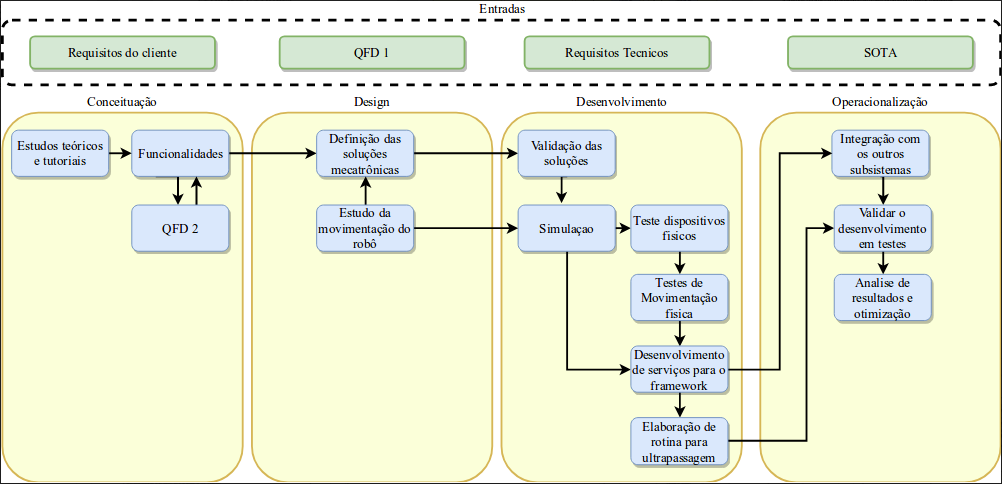
\includegraphics[scale=0.45]{Figures/flux_desen.png}
	\caption{Fluxograma de desenvolvimento}
	\label{fig:flux_desen}
\end{figure}	

Devido a complexidade envolvida nesse tipo de sistema, são utilizadas ferramentas específicas de desenvolvimento, assim como o cliente fornece certos parâmetros iniciais para impulsionar o projeto e guiar desenvolvimento para um resultado satisfatório. São consideradas entradas para a metodologia os requisitos do cliente, requisitos técnicos, um \textit{QFD} inicial, denominado \textit{QFD} 1 e o Estudo do Estado da Arte (\textit{SOTA}).


O requisito consiste na definição documentada  de uma propriedade ou comportamento que um produto ou serviço particular deve atender. Existem os requisitos do cliente, no qual são as necessidades e as expectativas do cliente, e os requisitos técnicos possui uma visão técnica para atender as necessidades do cliente e os objetivos do projeto.

Durante a fase inicial do projeto, foi conversado com o cliente e deixado explícito seus requisitos para o \textit{ELIR}, sendo eles:

\begin{itemize}
	\item Realizar as funções de forma autônoma;
	
	\item Transpor obstáculos e cadeia de isoladores;
	
	\item Deslocar-se através do consumo de baterias;
	
    \item Deslocamento/movimento realizada por servomotores.
    
\end{itemize}

Foi determinado pelo cliente para que o projeto desempenhe corretamente os seguintes requisitos técnicos:
\begin{itemize}
	\item Desempenho de deslocamento de 15km por dia
	
	
	\item Velocidade de deslocamento médio  sem obstáculos de 0.5 m/s
	
	
	\item Ultrapassagem de obstáculos de volume máximo de  410x330x150mm
	
	\item Autonomia de potência de 2 horas
    \item Sistema operacional Linux, 
	\item \textit{Backend} em C++ e Python
	\item \textit{Framework} ROS Kinetic Kame.
	
	
\end{itemize}

A ferramenta de Desdobramento da Função Qualidade (\textit{QFD}) torna-se importante para guiar o projeto e a incorporar as reais necessidades do cliente.  Por meio de um conjunto de matrizes parte-se dos requisitos expostos pelos clientes e realiza-se um processo de "desdobramento" transformando-os em especificações técnicas do produto. Esse desdobramento entre os requisitos do cliente, influencia no desenvolvimento, permitindo encontrar o que impacta mais no resultado final do projeto, assim fazendo com que a prioridade de certas atividades mude.

O estudo do estado da arte é o mapeamento que possibilitará o conhecimento e/ou reconhecimento de estudos que estão sendo, ou já foram realizados com temáticas, ou linhas de pesquisa , iguais ou parecidas a que está sendo estudando. No caso de projetos desenvolvidos em conjunto que incorporam diversas teses acadêmicas, esse estudo facilita a continuação do trabalho e dá uma base o projeto.

%--------- NEW SECTION----------------------
\section{Conceituação}
\label{sec:conc}
A fase da conceituação consiste na criação de um conceito para o sistema, sendo assim recolhido todo o embasamento teórico necessário para a confecção do projeto. Assim fazendo com que seja elaborada uma ideia para o sistema, o que é a base para todo o projeto, guiando as próximas fases.

As entradas do cliente são de suma importância para essa etapa, onde as mesmas são a base para a ideia do sistema. Com o estudo teórico do que será necessário e o uso das ferramentas como o \textit{QFD}, é possível elaborar as funcionalidades que serão desempenhadas pelo sistema. A elaboração de um segundo \textit{QFD} por parte da equipe acontece em paralelo com a elaboração das funcionalidades e se utiliza do \textit{QFD} 1 junto com os requisitos técnicos e do cliente, buscando conceituar o sistema de forma concreta.

As funcionalidades recebem entradas e saídas, sendo assim, interligadas, esse tipo de metodologia se mostra muito eficiente pois consegue dividir o robô em subsistemas e funções a serem desempenhadas, podendo assim dar uma idéia de como será o seu funcionamento e troca de informações internas. Com a definição das funcionalidades do sistema, é possível partir para a forma da idéia, como ela será aplicada, o que acontece na etapa de \textit{Design};  


\section{\textit{Design}}
\label{sec:design}
Com um conceito firme para o sistema, a etapa de \textit{design} consiste na forma que a idéia irá ter, para que a mesma seja possível. Com as funcionalidades definidas, é possível decidir quais ferramentas devem ser utilizadas no projeto, de forma a garantir que as mesmas sejam executadas. 

Por se tratar do desenvolvimento de um sistema de movimentação, é importante que seja realizado um estudo da forma como será necessário se realizar o movimento do robô, já que isso impacta profundamente na seleção das ferramentas, esse estudo consiste na busca do entendimento de como será sua aplicação real, e está relacionado também com a simulação, que colabora para o sucesso dessa etapa. São tomados como critérios para a escolha da ferramentas: A quantidade de informação sobre cada ferramenta que há disponível, suporte da comunidade que a utiliza e os tutoriais que cada ferramenta possui. O estudo da movimentação é de grande valia no \textit{design} das soluções mecatrônicas pois, conhecendo as maneiras quais o robô tem que se movimentar, definir os recursos necessários para esse objetivo se torna mais fácil.

\section{Desenvolvimento}
\label{sec:Desen}
O desenvolvimento consiste na aplicação prática da idéia, sendo a parte que demanda mais tempo e a partir dela, já é possível ter a noção de como será o dispositivo físico final. Contém toda a produção de software, estruturas necessárias para o projeto, e também a construção do protótipo. Com a definição das ferramentas realizada na etapa de \textit{design}, é possível começar a aplicação no sistema de interesse, validando o que foi decidido anteriormente.

\subsection{Validação das ferramentas}
\label{ssec:val_ferra}
A etapa de validação das ferramentas é onde se realiza os estudos e testes para compreender o funcionamento das mesmas e verificar se suas mecânicas e funcionalidades são adequadas para a solução e desenvolvimento do projeto. Uma vez que a ferramenta esteja escolhida, é realizada a análise do seu funcionamento, seus aspectos gerais, configurações, e como integrá-las ao desenvolvimento do projeto.

Após realizado o estudo da ferramenta, e de como suas mecânicas funcionam e podem auxiliar no desenvolvimento das funcionalidades do projeto, são realizados os primeiros usos das ferramentas, por meio de pequenos testes específicos, a fim de buscar o entendimento amplo de como se operacionalizar e implementar as soluções a partir das funcionalidades das ferramentas. 

Uma vez que os testes se mostram efetivos e o conhecimento sobre as suas funcionalidades esteja adquirido, a ferramenta torna-se válida, e pode ser utilizada no desenvolvimento do projeto, podendo ser utilizada em todas as etapas onde se mostre necessária

\subsection{Movimentação simulada/em simulação}
\label{ssec:mov_sim}
Para a validação das ferramentas, o uso de simulações computacionais é fundamental, devido que a simulação consegue prever os comportamentos do protótipo antes do mesmo estar em operação e com uso das ferramentas disponíveis na robótica e assim validando a maioria das ferramentas e estratégias. A simulação torna-se presente em todos os testes, desde a validação de ferramentas definidas durante a fase de \textit{Design} até do robô em operação, sendo uma poderosa ferramenta para validação dos dispositivos e a movimentação física.

\subsection{Teste com dispositivos físicos e Movimentação física}
\label{ssec:test_fis}
Antes de realizar testes do robô se movimentando é necessário garantir que todos os dispositivos físicos estejam funcionando corretamente. Durante essa fase deverá ser realizado a montagem do robô e garantir que esteja conforme a simulação. Logo após, é de extrema importância realizar simulações, testes de esforço, velocidades e posição dos servomotores utilizados na estrutura para que não haja nenhum imprevisto durante os próximos testes de operação. 

Com os testes de dispositivos físicos realizados unitariamente, é necessário integrá-los para realizar os testes de movimentação física. Esse teste é realizado tanto na simulação quanto em operação em linha, sendo importante verificar se o mesmo está andando corretamente, observando influência externa do vento. 

\subsection{Desenvolvimento de serviços para \textit{framework} e rotina para ultrapassagem}
\label{ssec:serv_ultr}
A estrutura de serviços disponibilizada pelo \textit{framework}, são subrotinas em código para desempenhar uma função específica, a comunicação é feita por um par de mensagens, uma de solicitação e outra de resposta, que quando necessário fazer uso do serviço, uma mensagem de solicitação é enviada, logo após o serviço executa o código contigo nele e retorna uma mensagem de resposta. 

Para realizar o rotina de ultrapassagem como um todo é conveniente separar em serviços as partes dos movimento de ultrapassagem, facilitando a identificação de erros e inconsistências. Com os serviços feitos e testados é preciso unificá-los para realizar a ultrapassagem. É importante organizá-los de forma sequencial e analisar como cada serviço se comporta para garantir que foram bem codificados, e se necessário realizar ajustes na programação. 

\section{Operacionalização}
\label{sec:operal}
A operacionalização põe em funcionamento todo o conjunto dos dispositivos, sistemas e rotinas necessárias para o funcionamento do robô. A partir do momento em que há itens, rotinas e ferramentas que são parte de uma funcionalidade, desenvolvidas, passa a ser possível a junção destes para que essa funcionalidade tome forma. Com estas finalizadas, é realizada sua integração com outras funcionalidades, para que possa receber suas entradas e entregar suas saídas.

Deve-se também verificar o desempenho das funcionalidades, a validação do desenvolvimento é realizada com testes de operação dos sistemas. Nestes testes, são executados procedimentos que repliquem as situações de operação do robô. É importante também que as condições dessa operação, ambiente, carga e etc. sejam similares as quais o robô irá encontrar.

Após a realização de testes para a validação do desenvolvimento, é possível analisar os resultados dos mesmos. As informações levantadas nos testes mostram se as funcionalidades desenvolvidas realizam o que se espera e a sua eficiência. A partir daí, pontos do projeto a serem melhorados ficam evidentes, possibilitando assim a otimização de funções.
